\documentclass[12pt]{article}

\usepackage{url}
\usepackage{fullpage}
\usepackage{amssymb,amsfonts}
\usepackage{amsmath}
\newcommand{\eps}{\varepsilon}
\newcommand{\R}{\mathbb{R}}

\usepackage{listings}
\usepackage{color}
\usepackage{graphicx}

\usepackage{varwidth}

\usepackage{hyperref}
\hypersetup{
    linktoc=all,     %set to all if you want both sections and subsections linked
    colorlinks=true,
    linkcolor=blue,
    filecolor=magenta,      
    urlcolor=cyan,
}

\definecolor{dkgreen}{rgb}{0,0.6,0}
\definecolor{gray}{rgb}{0.5,0.5,0.5}
\definecolor{mauve}{rgb}{0.58,0,0.82}

\lstset{frame=tb,
  language=Python,
  aboveskip=3mm,
  belowskip=3mm,
  showstringspaces=false,
  columns=flexible,
  basicstyle={\small\ttfamily},
  numbers=none,
  numberstyle=\tiny\color{gray},
  keywordstyle=\color{blue},
  commentstyle=\color{dkgreen},
  stringstyle=\color{mauve},
  breaklines=true,
  breakatwhitespace=true,
  tabsize=3
}

\usepackage[toc,page]{appendix}

\DeclareMathOperator*{\E}{\mathbb{E}}
\let\Pr\relax
\DeclareMathOperator*{\Pr}{\mathbb{P}}

\def\cl{\lstinline}

\title{CS 208 Homework 1}
\author{Andrew Shackelford}
\date{February 26, 2019}
\setcounter{tocdepth}{3}

\begin{document}

\maketitle

\textbf{All code and figures are available \href{https://github.com/andrew-shackelford/cs208/tree/master/1}{here}}.

{
  \hypersetup{linkcolor=black, hidelinks}
  \tableofcontents
}

\newpage

\section{Problem 1}

\subsection{Process}

\noindent

In order to carry out a hypothetical reidentification attack against the PUMS dataset, we need to figure out how unique our population is when we have access to certain combinations of attributes. The code for this attack, \cl{problem_1_attack.py}, is available at Appendix \ref{appendix:problem_1_attack}.

\subsubsection{Calculating Population Proportions}

\noindent

First, we will analyze the characteristics of our $5\%$ sample. To do so, we will count how often each different value of a variable occurs for each attribute. The code to calculate these counts is in the \cl{get_counts()} function.

\medskip

Once we have the counts, we will calculate the proportions for each characteristic using the \cl{get_proportions()} function.

\subsubsection{Generating Random Individuals}

\noindent

While we could have simply counted the number of unique individuals in the sample, our problem lies in the fact that the sample is only a $5\%$ random sample of the population. Therefore, we need to find the number of unique individuals out of a group of $20 \cdot n$ individuals, where $n$ is the number of individuals in the sample. In order to do this, we will generate $20n$ ``random'' individuals that match the characteristics of our sample. The code to do this is in the \cl{generate_random_individuals()} function.

\medskip

Once we generate those individuals that match the characteristics of our sample, we simply need to count the number of unique ones, and report that number. This code is in the appropriately named \cl{count_unique_individuals()} function.

\subsubsection{Trying Different Attacks}

\noindent

I tried several different combinations of demographic attributes in order to see which ones would be effective at reidentification attacks. These combinations included:

\begin{itemize}
  \item \textit{Attack A:} attributes based on only publicly available information
  \begin{itemize}
    \item sex
    \item race
    \item marital status
  \end{itemize}
  \item \textit{Attack B:} attributes based on publicly available information and information that would be available from an individual's tax return
  \begin{itemize}
    \item sex
    \item race
    \item marital status
    \item PUMA (derived from address)
    \item children
    \item employment status
    \item income
  \end{itemize}
  \item \textit{Attack C:} attributes based on publicly available information and information that would be available from a voter registration database
  \begin{itemize}
    \item sex
    \item race
    \item marital status
    \item PUMA (derived from address)
    \item age (derived from birthdate)
  \end{itemize}
  \item \textit{Attack D:} attributes based on publicly available information and information that would be available from an individual's tax return and voter registration database
  \begin{itemize}
    \item sex
    \item race
    \item marital status
    \item PUMA (derived from address)
    \item children
    \item employment status
    \item income
    \item age (derived from birthdate)
  \end{itemize}
\end{itemize}

\subsubsection{Caveat}

\noindent

However, this entire proposed attack depends on one crucial assumption: that each variable is independent of the rest. In the real world, race and age are correlated with income, race is likely correlated with address and therefore PUMA, and of course, children is highly correlated with marital status, not to mention countless other possible correlations. Therefore, the following calculations are likely optimistic, and in the real world less of the population would be unique due to the correlation of certain attributes. That being said, the following results are valid given that crucial assumption.

\subsection{Results}

\noindent

\begin{tabular}{|c|c|c|}
\hline
Attack Type & Number Reidentified & Success Rate \\ \hline
\textit{A} & 0 & 0 \\ \hline
\textit{B} & 115669 & 0.224 \\ \hline
\textit{C} & 3816 & 0.007 \\ \hline
\textit{D} & 394208 & 0.765 \\ \hline
\end{tabular}

\subsection{Analysis}

\noindent

Examining our results, we find that only using publicly available data, we would not be able to reidentify any individuals in the dataset. If we had access to a voter registration database, assuming each individual in the database had registered to vote, we'd be able to reidentify 3816 individuals, or approximately $0.7\%$ of the dataset.

\medskip

If, however, we were able to gain access to a more private source of data, such as an individual's tax return, we'd be able to identify $22.4\%$ of the dataset, and lastly, if we had access to both a tax return and a voter registration database, we'd be able to identify an astoundingly high $76.5\%$ of the dataset.

\medskip

All of this analysis, however, is still predicated on the assumption that each variable is independent of the rest, something that is unlikely if not completely false in the real world. If the variables were dependent on one another, as they are in the real world, the success rate would likely drop for each of the various reidentification attacks. This attack also would also depend on having access to something like an individual's tax return, which is already a fairly sensitive document to gain access to. However, given those two caveats, we have proposed a very successful reidentification attack.

\newpage

\section{Problem 2}

\subsection{Process}

\noindent

In order to determine how well this reconstruction attack performs on different defenses, I used a Python script that ran experiments with various defenses and parameters and wrote out the results to a CSV file. The code, \cl{problem_2_attack.py}, is available at Appendix \ref{appendix:problem_2_attack}.

\medskip

Once the experiments finished, I graphed the results using Python's \cl{matplotlib} library. The code, \cl{problem_2_graph.py}, is available at Appendix \ref{appendix:problem_2_graph}.

\subsection{Plots}

\noindent

Below are the plots produced for each of the defense strategies, both for the overall success rate and the root-mean-squared-error for each parameter.

\subsubsection{Rounding}
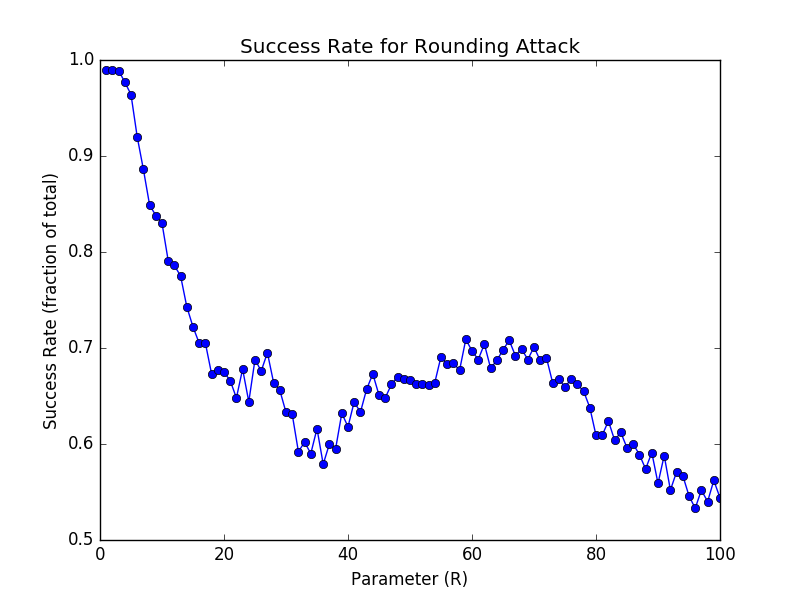
\includegraphics[scale=0.4]{figures/problem_2_rounding_success_rate.png} 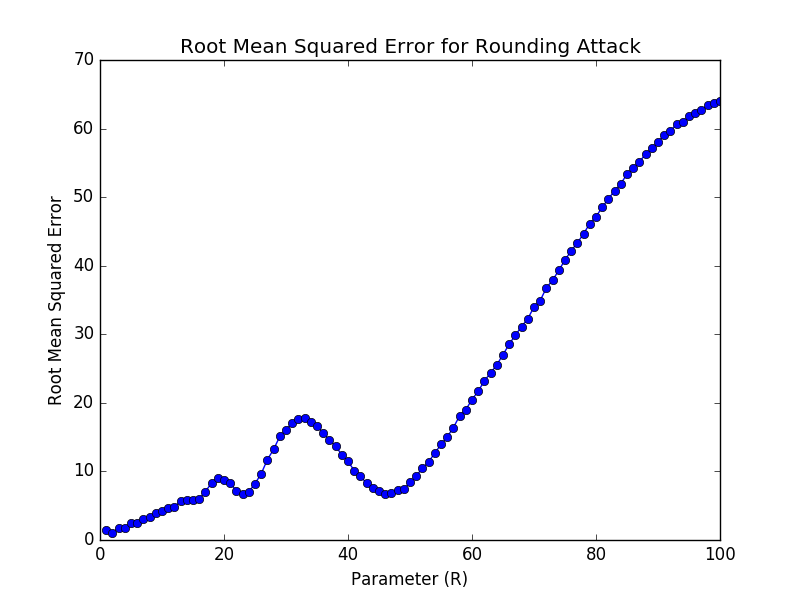
\includegraphics[scale=0.4]{figures/problem_2_rounding_error.png}

\subsubsection{Noise Addition}
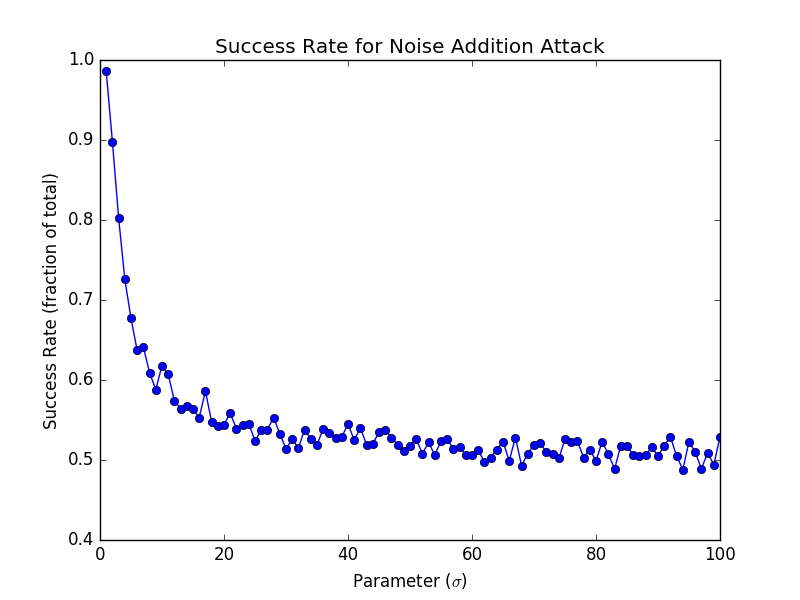
\includegraphics[scale=0.4]{figures/problem_2_noise_addition_success_rate.png} 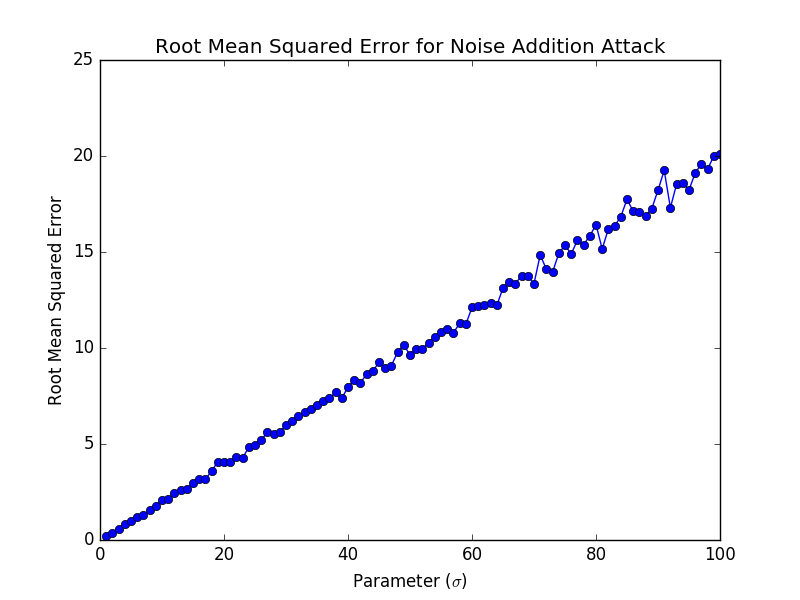
\includegraphics[scale=0.4]{figures/problem_2_noise_addition_error.png} 

\subsubsection{Subsampling}
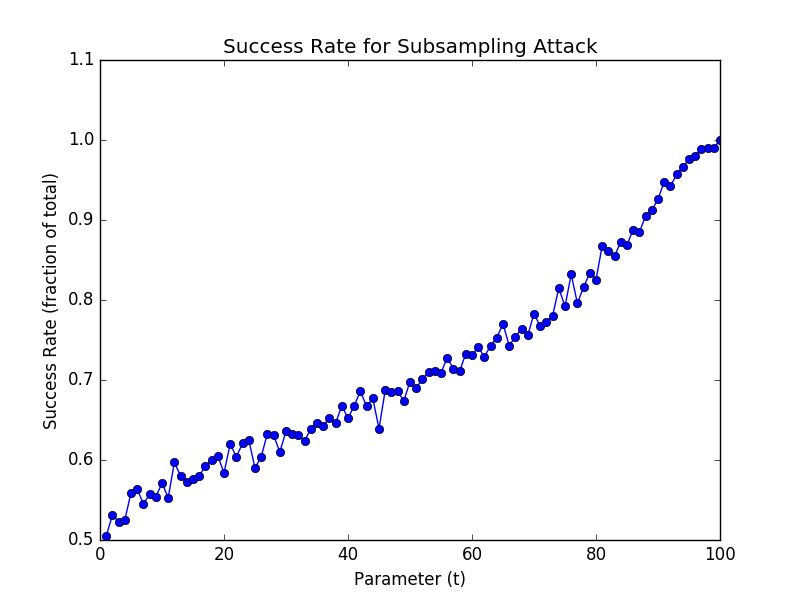
\includegraphics[scale=0.4]{figures/problem_2_subsampling_success_rate.png} 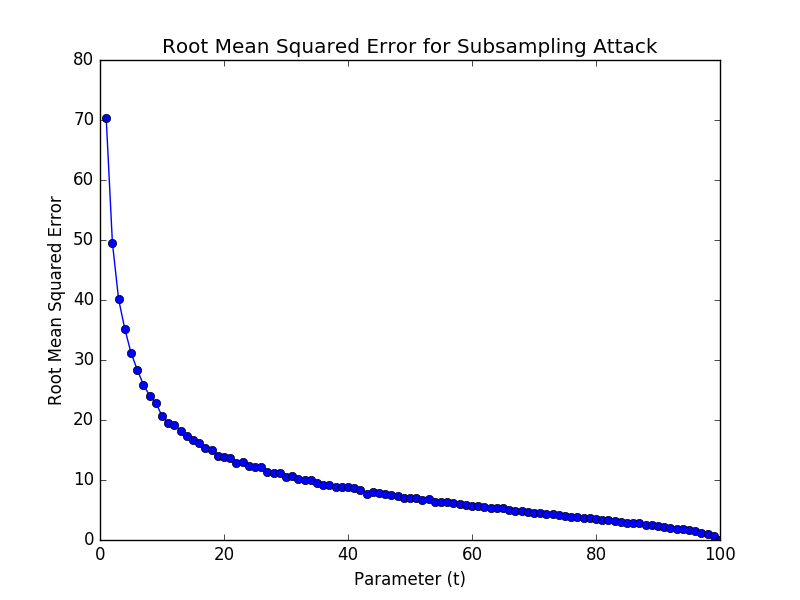
\includegraphics[scale=0.4]{figures/problem_2_subsampling_error.png} 

\subsection{Analysis}

\noindent

Unsurprisingly, we notice that as we increase the strength of each defense's parameter, the reconstruction success rate drops.

\subsubsection{Rounding}

\noindent

For the rounding defense, we notice a steep decline in success rate until $R = 40$, a slight increase until $R = 65$, and then a continued decrease as $R$ continues to increase. Curiously, the RMSE metric does not directly correlate with the success rate. While the success rate is a full 10 percent higher at $R = 60$ than $R = 40$, the RMSE is actually higher. Regardless, the attack's success rate falls below 60 percent at approximately $R = 35$, and approaches 50 percent at $R = 90$.

\subsubsection{Noise Addition}

\noindent

For the noise addition defense, we notice an exponential-like curve for the success rate, and a linear graph for the RMSE. It does not take a high value of $\sigma$ for the noise addition attack to prevent reconstruction - a value of $\sigma = 10$ causes the success rate to fall below 60 percent, and $\sigma = 30$ is sufficient to cause approximately 50 percent of the reconstruction attempts to fail.

\subsubsection{Subsampling}

\noindent

Before we begin our analysis, it is important to note for that for the subsampling defense low values of $t$ are extreme, i.e. $t = 100$ implies no defense at all. For the subsampling defense, we see a linear increase in success rate as we increase the size of the subsample, and a exponential-like curve on the RMSE metric. Like the rounding defense, this defense requires a relatively extreme parameter to cause the attack to become unsuccessful - only once $t \leq 20$ does the success rate fall below 60 percent. Even at the most extreme $t = 1$ does the success rate barely approach 50 percent.

\subsubsection{Summary}

\noindent

Of these three defense strategies, the noise addition appears to be the most successful at preventing reconstruction for a less extreme value of its parameter. Requiring only a value of $\sigma = 10$ for the success rate to consistently fall below 60 percent, this fares much better than $R = 80$ and $t = 20$ (where $t = 20$ is the $80\%$ most extreme defense). In addition, while the noise addition defense hits a success rate of $50\%$ around $\sigma = 20$, the other attacks don't reach that low of a success rate until the parameters reach their absolute extremes, $R = 100$ and $t = 1$, respectively. At such a point, the results from these queries yield almost no actionable data since there is so much inaccuracy in the result.

\medskip

It is worth noting, however, that all of these defenses have similar values of RMSE at their 60 percent and 50 percent thresholds. The simple difference is that the rounding defense, and to an extent the subsampling defense, cause systematic error while the noise addition defense will create a more uniform source of error.

\medskip

Based on these conclusions, it appears the noise addition defense is the best defense that reduces the success rate while preventing the results from being too inaccurate. As a result, when aiming to prevent reconstruction attacks while keeping the statistics useful, noise addition appears to be the best defense mechanism.

\newpage

\section{Problem 3}

\subsection{Process}

\subsubsection{Generating New Attributes}

\noindent

In order to have enough attributes to conduct a successful membership attack, I used a Python script to generate new attributes in the same method used in Problem 2. I chose to generate $n^2$ new attributes, so as to have plenty of attributes available depending on how many were needed in the attack. The new population and sample files were then written out to CSV files. I ended up only using $10n$ attributes, and simply splice off the rest each time upon loading. Once the new set of attributes were generated, I also calculated the sample and population means and stored those in separate CSV files to avoid having to recalculate them each time, as the full population file with $100^2$ attributes per person took up over a gigabyte of space. The code to generate these attributes, \cl{problem_3_attributes.py}, is available in Appendix \ref{appendix:problem_3_attributes}.

\subsubsection{Fixing Parameters}

\noindent

Now, we must fix parameters for each of our three defenses. Looking back at our results from Problem 2, we find that values $R = 35$, $\sigma = 10$, and $t = 20$ should be sufficient to cause less than 60 percent (approximately $\frac{1}{2}$) of the bits to be reconstructed.

\subsubsection{Performing Attack}

\noindent

Now that we have fixed the parameters, we'll slightly modify our code from Problem 2 to keep the attributes fixed while varying the number of queries, and see how the attack performs. The code to carry out this attack, \cl{problem_3_attack.py}, is availabile in Appendix \ref{appendix:problem_3_attack}.

\medskip

Once the experiments finished, I graphed the results using Python's \cl{matplotlib} library. Before I graphed them, I used \cl{np.convolve} to smooth out some of the noise in the data so the graphs would be more readable. The code to graph the results, \cl{problem_3_graph.py}, is available at Appendix \ref{appendix:problem_3_graph}.

\subsection{Plots}

\noindent

Below are the plots produced for each of the defense strategies, with the number of queries on the x-axis and the true positive rate on the y-axis.

\subsubsection{Rounding}
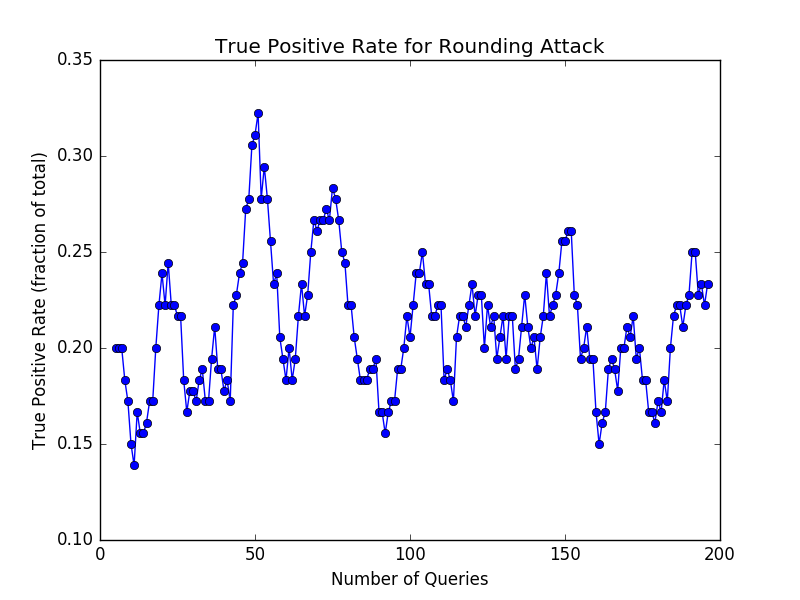
\includegraphics[scale=0.6]{figures/problem_3_rounding_true_positive_rate.png}

\subsubsection{Noise Addition}
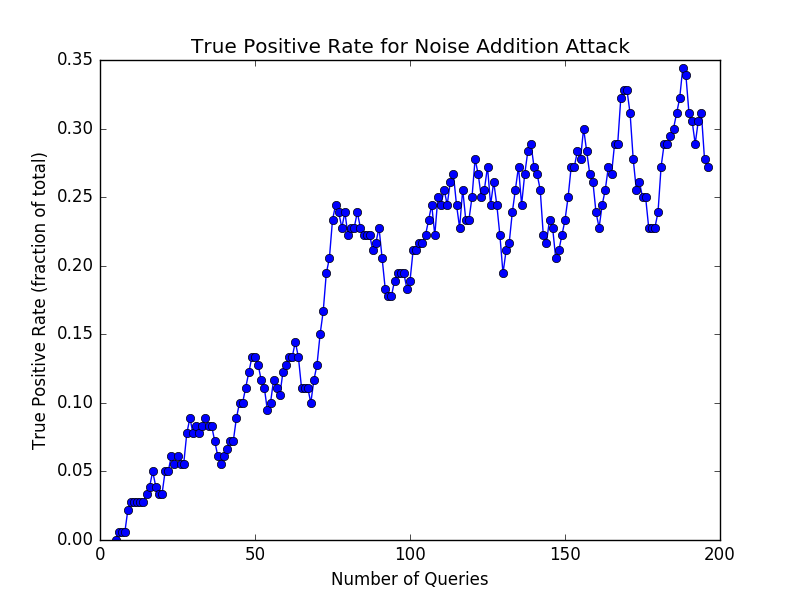
\includegraphics[scale=0.6]{figures/problem_3_noise_addition_true_positive_rate.png}

\subsubsection{Subsampling}
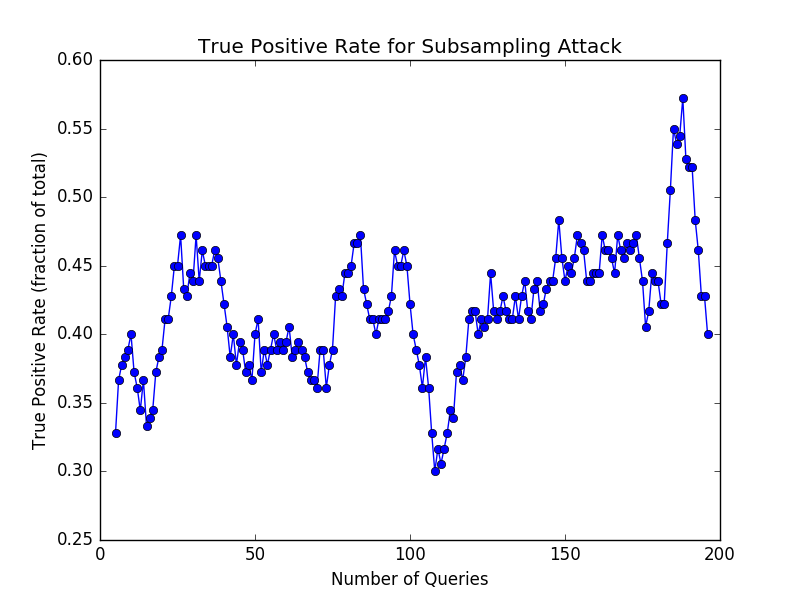
\includegraphics[scale=0.6]{figures/problem_3_subsampling_true_positive_rate.png}

\newpage

\subsection{Analysis} 

\subsubsection{Rounding Defense}

\noindent

In regards to the rounding defense, the most important thing to note is that increasing the number of queries will have no impact on the results returned by the rounding attack, since each query is going to round to the same number anyway. As a result, the only factor is the parameter that we fixed earlier, which was $R = 35$. Since we're rounding a sample of 100 to the nearest multiple of 35, there is very little information to be gleaned from this data, and increasing the number of queries is not going to affect the success rate of the attack, since each query will be rounded to the same number anyways. Therefore, it makes sense that the membership attack against the rounding defense would not perform that well and not be correlated with the number of queries.

\subsubsection{Noise Addition Defense}

\noindent

The membership attack fares much better against the noise addition defense. While small numbers of queries are unsuccessful, we can see a clear and steady increase in true positive rate as we increase the number of queries, reaching a consistent 30 percent true positive rate once the number of queries is greater than 10, and a consistent 35 percent true positive rate once the number of queries is greater than 35. At points, the true positive rate even approaches 50 percent. This shows the vulnerability that repeated queries can have on simple noise addition defenses.

\subsubsection{Subsampling Defense}

\noindent

The membership attack also has good results against the subsampling defense. The true positive rate is always above 30 percent and only rarely dips below 35 percent. In fact, it holds around 45 percent on average, and at certain points we obtain a true positive rate as high as 50 percent.

\subsubsection{False Positive Rate}

\noindent

While we have shown that our attack has a fairly high true positive rate, we must also ensure that it does not have too high of a false positive rate. In order to ensure we have a false positive rate of $\frac{1}{10n}$, we set our p-value = 0.001. In order to test the false positive rate, we fix our number of queries to be $2n$ against our noise addition defense. Running a test of 1000 queries on a previously generated random subset of the population known not to be in the sample, we found 0 false positives, thus confirming that our false positive rate is empirically $\leq \frac{1}{10n}$. The code to execute this attack is also available in the \cl{false_positive_rate()} function of \cl{problem_3_attack.py}, and is located at Appendix \ref{appendix:problem_3_attack}.

\subsubsection{Summary}

\noindent

These results show that even when we reach the point where reconstruction attacks are no longer viable, we can execute a membership attack against the same dataset with fairly good results, obtaining best case true positive rates of anywhere from 30 percent to 45 percent, depending on the defense mechanism used. However, this attack does not work against the rounding defense, simply because additional queries do not lend us additional information about the dataset. In addition, these results show that we can perform such a membership attack with a very low false positive rate as well, thus giving us useful data about whether a specific member of the population is definitely in the sample. During testing, I performed the same membership attack with a p-value of 0.05 and found true positive rates of approximately 80 percent. As a result, it appears that if we were willing to accept higher false positive rates, we could obtain much higher true positive rates as well.

\newpage

\section{Problem 4}

\noindent

I have a few different ideas on possible final project topics. First, I'd be interested in creating a differentially private querying system for the Census data from this problem set, that makes the reconstruction and membership attacks infeasible. This would be an experimental project where I would develop a differentially private querying mechanism and test both its effectiveness at preventing privacy leaks and measure the error introduced by the mechanism.

\bigskip

I'd also be interested in developing an attack against an existing database. I'd be especially curious about attacking a database in some way related to Harvard, since that would both demonstrate the effect privacy leaks have on our community and perhaps afford us a chance to fix it. However, I haven't been able to think of any databases that fill these criteria yet, and would be open to suggestions from the professors. In this case, I anticipate developing a kind of reconstruction or membership attack against such database and then proposing, and perhaps implementing, methods to fix the privacy leaks found.

\newpage

\begin{appendices}

\section{\cl{problem_1_attack.py}}
\label{appendix:problem_1_attack}

\begin{lstlisting}
"""
Andrew Shackelford
ashackelford@college.harvard.edu

CS 208 - Spring 2019
Homework 1, Problem 1
"""

import csv
import numpy as np
from collections import Counter

TOTAL = 25766 * 20 # number of rows in 5% sample * 20 to get total

# load and clean sample csv
def read_csv(file):
    with open(file, 'rU') as csv_file:
        reader = csv.DictReader(csv_file)
        data = []
        for row in reader:
            if row['englishability'] == 'NA':
                row['englishability'] = 2
            if row['income'][-4:] == 'e+05':
                row['income'] = int(row['income'][:-4]) * 100000
            for key in row.keys():
                row[key] = int(row[key])
            data.append(row)
        return data

# count number of entries with each possible value
def get_counts(data):
    ret = {}
    for row in data:
        for key, value in row.iteritems():
            entry = ret.get(key, {})
            entry[value] = entry.get(value, 0) + 20 # use 20 instead of 1, since 5% sample
            ret[key] = entry
    return ret

# convert counts to proportions
def get_proportions(counts):
    for attr, breakdown in counts.iteritems():
        for value, number in breakdown.iteritems():
            breakdown[value] = float(number) / float(TOTAL)
    return counts

# generate new random individuals with properties of dataset
def generate_random_individuals(proportions, desired_attributes):
    generated = ["" for i in range(TOTAL)]

    # for each attribute
    for attr, breakdown in proportions.iteritems():
        # that we plan to use in our reconstruction attack
        if attr not in desired_attributes:
            continue

        # get the possible options as well as the proportions for each option
        keys = breakdown.keys()
        values = breakdown.values()

        # represent each individual as a concatenated string of each attribute
        for idx, individual in enumerate(generated):
            generated[idx] = individual + str(np.random.choice(keys, p=values))

    return generated

# count the number of individuals that are unique
def count_unique_individuals(generated):
    counter = Counter(generated)
    num_unique = 0
    for element, number in counter.most_common():
        if number == 1:
            num_unique += 1
    return num_unique

def main():
    data = read_csv('FultonPUMS5full.csv')
    counts = get_counts(data)
    proportions = get_proportions(counts)

    # attributes based on only publicly available information
    desired_attributes = ['sex', 'latino', 'black', 'asian', 'married', 'divorced']
    generated = generate_random_individuals(proportions, desired_attributes)
    print(count_unique_individuals(generated))

    # attributes based on tax returns
    desired_attributes = ['sex', 'latino', 'black', 'asian', 'married', 'divorced', 'puma', 'children', 'employed', 'income']
    generated = generate_random_individuals(proportions, desired_attributes)
    print(count_unique_individuals(generated))

    # attributes based on voter registration database
    desired_attributes = ['sex', 'latino', 'black', 'asian', 'married', 'divorced', 'puma', 'age']
    generated = generate_random_individuals(proportions, desired_attributes)
    print(count_unique_individuals(generated))

    # attributes based on tax returns + voter registration database
    desired_attributes = ['sex', 'latino', 'black', 'asian', 'married', 'divorced', 'puma', 'children', 'employed', 'income', 'age']
    generated = generate_random_individuals(proportions, desired_attributes)
    print(count_unique_individuals(generated))

if __name__ == "__main__":
    main()
\end{lstlisting}

\newpage

\section{\cl{problem_2_attack.py}}
\label{appendix:problem_2_attack}

\begin{lstlisting}
"""
Andrew Shackelford
ashackelford@college.harvard.edu

CS 208 - Spring 2019
Homework 1, Problem 2
"""

import numpy as np
from scipy import stats
import math
import csv
import progressbar

# public attributes
PUB = ['sex',
       'age',
       'educ',
       'married',
       'divorced',
       'latino',
       'black',
       'asian',
       'children',
       'employed',
       'militaryservice',
       'disability',
       'englishability']

# defense strategies
ROUNDING = 1
NOISE_ADDITION = 2
SUBSAMPLING = 3

# prime number
P = 773

# load and clean sample csv
def read_csv(file):
    with open(file, 'rU') as csv_file:
        reader = csv.DictReader(csv_file)
        data = []
        for row in reader:
            if row['englishability'] == 'NA':
                row['englishability'] = 2
            if row['income'] == '1e+05':
                row['income'] = 100000
            for key in row.keys():
                row[key] = int(row[key])
            data.append(row)
        return data

# perform a query with no defense
def get_query(data, predicate):
    result = 0.
    x = np.zeros(len(data))
    for idx, row in enumerate(data):
        if predicate(row):
            result += row['uscitizen']
            x[idx] = 1.
    return result, x

# perform a subsampled query
def get_subsampled_query(data, predicate, subsample_indices):
    result = 0.
    x = np.zeros(len(data))
    for idx, row in enumerate(data):
        if predicate(row):
            x[idx] = 1.
            if idx in subsample_indices:
                result += row['uscitizen']
    return result, x

# perform a query with rounding defense
def rounding(data, predicate, R):
    result, x = get_query(data, predicate)
    modulo = result % R
    if (modulo < R/2):
        return result - modulo, x
    else:
        return result + (R - modulo), x

# perform a query with noise addition defense
def noise_addition(data, predicate, sigma):
    result, x = get_query(data, predicate)
    result = result + np.random.normal(scale=sigma)
    return result, x

# perform a query with subsampling defense
def subsampling(data, predicate, t):
    subsample_indices = set(np.random.choice(len(data), size=t, replace=False))
    result, x = get_subsampled_query(data, predicate, subsample_indices)
    scale_factor = float(len(data)) / float(t)
    return result * scale_factor, x

# perform a query with various defense types and parameters
def query(data, predicate, defense_type=0, defense_factor=0.):
    if (defense_type == SUBSAMPLING):
        return subsampling(data, predicate, defense_factor)
    elif (defense_type == NOISE_ADDITION):
        return noise_addition(data, predicate, defense_factor)
    elif (defense_type == ROUNDING):
        return rounding(data, predicate, defense_factor)
    else:
        return get_query(data, predicate)

# generate a random vector for use in creating random subsets
def gen_random_vector(length):
    global random_vector
    random_vector = []
    for i in range(length):
        random_vector.append(np.random.randint(P))

# a random predicate to generate random subsets
def random_predicate(row):
    global random_vector
    sum = 0
    for idx, pub_key in enumerate(PUB):
        sum += random_vector[idx] * row[pub_key]
    return (sum % P) % 2 == 1

# run an experiment given data, n, a defense type and parameter
def experiment(data, n, defense_type, defense_factor):
    experiment_bar = progressbar.ProgressBar(maxval=2*n,
                                             widgets=[progressbar.Bar('=', '[', ']'),
                                             ' ',
                                             progressbar.Percentage()])
    experiment_bar.start()

    # reset total squared error
    total_squared_error = 0.

    # perform 2n queries
    for i in range(2*n):
        experiment_bar.update(i)

        gen_random_vector(len(PUB)) # generate a new subset for each query

        y, x = query(data, random_predicate, defense_type, defense_factor)
        truth, _ = query(data, random_predicate)

        total_squared_error += np.square(y - truth) # calculate error

        if i == 0:
            Ys, Xs = y, x
        else:
            Ys, Xs = np.vstack((Ys, y)), np.vstack((Xs, x))

    experiment_bar.finish()

    # perform least squares regression
    Betas, residuals, ranks, s = np.linalg.lstsq(Xs, Ys)

    # calculate number of successes
    successes = 0
    false_positives = 0
    false_negatives = 0
    for index, estimate in enumerate(Betas):
        if estimate >= 0.5:
            if data[index]['uscitizen']:
                successes += 1
            else:
                false_positives += 1
        else:
            if data[index]['uscitizen']:
                false_negatives += 1
            else:
                successes += 1

    # calculate success rate
    success_rate = float(successes) / float(len(data))

    # calculate root mean squared error
    mse = total_squared_error / float(n)
    root_mse = math.sqrt(mse)

    # create an output row for the csv
    output = [defense_type,
              defense_factor,
              successes,
              false_positives,
              false_negatives,
              success_rate,
              root_mse]

    return output

def main():
    # read in the 100-person sample
    data = read_csv('FultonPUMS5sample100.csv')
    n = len(data)

    # write out the results to a csv file
    with open('problem_2_results.csv', 'wb') as out_csv:
        writer = csv.writer(out_csv)
        writer.writerow(['defense_type',
                         'defense_factor',
                         'successes',
                         'false_positives',
                         'false_negatives',
                         'success_rate',
                         'root_mse'])

        # iterate through each defense type and parameter
        for defense_type in range(1, 4):
            for defense_factor in range(1, n+1):
                defense_factor = int(defense_factor)
                print("defense_type: " + str(defense_type) + " with defense_factor " + str(defense_factor))
                average = np.zeros(7)
                for i in range(10): # run 10 trials
                    print("Trial " + str(i+1) + " of 10")
                    average += experiment(data, n, defense_type, defense_factor)
                average /= 10
                writer.writerow(average)

if __name__ == "__main__":
    main()
\end{lstlisting}

\newpage

\section{\cl{problem_2_graph.py}}
\label{appendix:problem_2_graph}

\begin{lstlisting}
"""
Andrew Shackelford
ashackelford@college.harvard.edu

CS 208 - Spring 2019
Homework 1, Problem 2
"""

import csv
import matplotlib.pyplot as plt

# defense strategies
ROUNDING = 1
NOISE_ADDITION = 2
SUBSAMPLING = 3

# read in result csv
def read_csv(file):
    with open(file, 'rU') as csv_file:
        reader = csv.DictReader(csv_file)
        rounding = []
        noise_addition = []
        subsampling = []
        for row in reader:
            if float(row['defense_type']) == ROUNDING:
                rounding.append(row)
            elif float(row['defense_type']) == NOISE_ADDITION:
                noise_addition.append(row)
            elif float(row['defense_type']) == SUBSAMPLING:
                subsampling.append(row)
        return rounding, noise_addition, subsampling

# plot result graph
def plot_graph(data, attributes):
    # load data
    x, y = [], []
    for row in data:
        x.append(float(row['defense_factor']))
        y.append(float(row[attributes['y_value']]))

    # plot data
    plt.plot(x, y, '-o')

    # set titles and labels
    if attributes['y_value'] == 'success_rate':     
        plt.title('Success Rate for ' + attributes['title'] + ' Attack')
        plt.xlabel('Parameter (' + attributes['parameter'] + ')')
        plt.ylabel('Success Rate (fraction of total)')
    else:
        plt.title('Root Mean Squared Error for ' + attributes['title'] + ' Attack')
        plt.xlabel('Parameter (' + attributes['parameter'] + ')')
        plt.ylabel('Root Mean Squared Error')

    # save to file and clear figure
    plt.savefig(attributes['output_file'])
    plt.clf()

def main():
    # read in results
    rounding, noise_addition, subsampling = read_csv('problem_2_results.csv')

    # plot graphs for different defense types and success rate / RMSE
    plot_graph(rounding, {
    'output_file' : 'figures/problem_2_rounding_success_rate.png',
    'title': 'Rounding',
    'parameter' : 'R',
    'y_value' : 'success_rate'
                         })

    plot_graph(rounding, {
    'output_file' : 'figures/problem_2_rounding_error.png',
    'title': 'Rounding',
    'parameter' : 'R',
    'y_value' : 'root_mse'
                         })

    plot_graph(noise_addition, {
    'output_file' : 'figures/problem_2_noise_addition_success_rate.png',
    'title': 'Noise Addition',
    'parameter' : r'$\sigma$',
    'y_value' : 'success_rate'
                               })

    plot_graph(noise_addition, {
    'output_file' : 'figures/problem_2_noise_addition_error.png',
    'title': 'Noise Addition',
    'parameter' : r'$\sigma$',
    'y_value' : 'root_mse'
                               })

    plot_graph(subsampling, {
   'output_file' : 'figures/problem_2_subsampling_success_rate.png',
   'title': 'Subsampling',
   'parameter' : 't',
   'y_value' : 'success_rate'
                            })
    
    plot_graph(subsampling, {
   'output_file' : 'figures/problem_2_subsampling_error.png',
   'title': 'Subsampling',
   'parameter' : 't',
   'y_value' : 'root_mse'
                            })

if __name__ == "__main__":
    main()
\end{lstlisting}

\newpage

\section{\cl{problem_3_attributes.py}}
\label{appendix:problem_3_attributes}

\begin{lstlisting}
"""
Andrew Shackelford
ashackelford@college.harvard.edu

CS 208 - Spring 2019
Homework 1, Problem 3
"""

import numpy as np
from scipy import stats
import math
import csv
import progressbar

# public attributes
PUB = ['sex',
       'age',
       'educ',
       'married',
       'divorced',
       'latino',
       'black',
       'asian',
       'children',
       'employed',
       'militaryservice',
       'disability',
       'englishability']

# prime number
P = 773

# random predicate generator
def random_predicate(row):
    sum = 0
    for idx, pub_key in enumerate(PUB):
        sum += np.random.randint(P) * row[pub_key]
    return (sum % P) % 2 == 1

# read and clean csv file
def read_csv(file):
    with open(file, 'rU') as csv_file:
        reader = csv.DictReader(csv_file)
        data = []
        for row in reader:
            if row['englishability'] == 'NA':
                row['englishability'] = 2
            if row['income'][-4:] == 'e+05':
                row['income'] = int(row['income'][:-4]) * 100000
            for key in row.keys():
                row[key] = int(row[key])
            data.append(row)
        return data

# generate m random attributes
def gen_attributes(row, m):
    result = []
    for i in range(m):
        if random_predicate(row):
            result.append(1.)
        else:
            result.append(0.)
    return result

# write derived attributes to csv file
def write_derived_attributes(sample, population):
    with open('problem_3_population.csv', 'wb') as pop_file:
        with open('problem_3_sample.csv', 'wb') as sam_file:
            attribute_bar = progressbar.ProgressBar(maxval=len(population),
                                                    widgets=[progressbar.Bar('=', '[', ']'),
                                                    ' ',
                                                    progressbar.Percentage(),
                                                    ' ',
                                                    progressbar.ETA()])
            attribute_bar.start()

            # create csv writers
            pop_writer = csv.writer(pop_file)
            sam_writer = csv.writer(sam_file)
            m = int(len(sample) ** 2.)

            # for each member of population, generate n^2 new attributes
            for idx, pop in enumerate(population):
                attribute_bar.update(idx)
                res = gen_attributes(pop, m)
                pop_writer.writerow(res)
                if pop in sample:
                    sam_writer.writerow(res)

            attribute_bar.finish()

def main():
    sample = read_csv('FultonPUMS5sample100.csv')
    population = read_csv('FultonPUMS5full.csv')
    write_derived_attributes(sample, population)

if __name__ == "__main__":
    main()
\end{lstlisting}

\newpage

\section{\cl{problem_3_attack.py}}
\label{appendix:problem_3_attack}

\begin{lstlisting}
"""
Andrew Shackelford
ashackelford@college.harvard.edu

CS 208 - Spring 2019
Homework 1, Problem 3
"""

import numpy as np
from scipy import stats
import math
import csv
import progressbar

# public keys
PUB = ['sex',
       'age',
       'educ',
       'married',
       'divorced',
       'latino',
       'black',
       'asian',
       'children',
       'employed',
       'militaryservice',
       'disability',
       'englishability']

# defense strategies
ROUNDING = 1
NOISE_ADDITION = 2
SUBSAMPLING = 3

# fixed defense parameters
ROUNDING_PARAM = 90
NOISE_ADDITION_PARAM = 40
SUBSAMPLING_PARAM = 10

# number of attributes to use
NUM_ATTRIBUTES = 1000

# prime number
P = 773

# sample and population lengths
SAMPLE_LEN = 100
POPULATION_LEN = 25766
POPULATION_SUBSET_LEN = 150

# false positive rate of 1/10n
P_VALUE = 1. / (10. * float(SAMPLE_LEN))

# read a csv file with just the means of the data
def read_mean_csv(file):
    with open(file, 'rU') as csv_file:
        reader = csv.reader(csv_file)
        for row in reader:
            return np.array(map(float, row[:NUM_ATTRIBUTES]))

# read a csv file with all rows of the data
def read_csv(file):
    with open(file, 'rU') as csv_file:
        data = []
        reader = csv.reader(csv_file)
        for row in reader:
            data.append(map(float, row[:NUM_ATTRIBUTES]))
        return np.array(data)

# perform a subsampled query
def get_subsampled_query(data, subsample_indices):
    result = np.zeros(len(data[0]))
    for idx, row in enumerate(data):
        if idx in subsample_indices:
            result += row
    return result

# perform a query with rounding defense
def rounding(data, R):
    result = np.zeros(len(data))
    for idx, val in enumerate(data):
        modulo = val % R
        if (modulo < R/2):
            result[idx] = val - modulo
        else:
            result[idx] = val + (R - modulo)
    return result

# perform a query with noise addition defense
def noise_addition(data, sigma):
    result = np.zeros(len(data))
    for idx, val in enumerate(data):
        result[idx] = val + np.random.normal(scale=sigma)
    return result

# perform a query with subsampling defense
def subsampling(data, t):
    subsample_indices = set(np.random.choice(len(data), size=t, replace=False))
    subsample = get_subsampled_query(data, subsample_indices)
    scale_factor = float(SAMPLE_LEN) / float(t)
    return subsample * scale_factor

# perform a query with various defense types and parameters
def query(data, defense_type=0):
    if (defense_type == SUBSAMPLING):
        return subsampling(data, SUBSAMPLING_PARAM) / SAMPLE_LEN
    elif (defense_type == NOISE_ADDITION):
        return noise_addition(data, NOISE_ADDITION_PARAM) / SAMPLE_LEN
    elif (defense_type == ROUNDING):
        return rounding(data, ROUNDING_PARAM) / SAMPLE_LEN
    else:
        return np.array(data) / SAMPLE_LEN

# test statistic as described in 2/8 lecture notes
def test_statistic(y, p, a):
    y_diff = y - p
    a_diff = a - p
    statistic = np.dot(y_diff, a_diff)
    variance = 0.
    for j in range(len(p)):
        variance += np.square(a[j] - p[j]) * p[j] * (1 - p[j])
    return statistic, variance

# perform experiment to determine true positive rate
def tpp_experiment(defense_type, num_queries, num_trials=20):
    global sample
    global sample_mean
    global sample_counts
    global population_mean
    global population_counts

    # count number of successes
    successes = 0

    # progress bar
    experiment_bar = progressbar.ProgressBar(maxval=num_trials,
                                         widgets=[progressbar.Bar('=', '[', ']'),
                                         ' ',
                                         progressbar.Percentage()])
    experiment_bar.start()

    # execute multiple trials to average
    for i in range(num_trials):
        experiment_bar.update(i)
        result_mean = np.zeros(len(sample_mean))

        # execute number of queries
        for _ in range(num_queries):
            if defense_type == SUBSAMPLING:
                result_mean += query(sample, defense_type)
            else:
                result_mean += query(sample_counts, defense_type)

        result_mean /= float(num_queries)

        # calculate test statistic and tail distance
        statistic, variance = test_statistic(
                              sample[np.random.randint(SAMPLE_LEN)],
                              population_mean,
                              result_mean)
        null_dst = stats.norm(0, math.sqrt(variance))
        percentile = null_dst.cdf(statistic)
        tail_distance = 0.5 - abs(percentile - 0.5)

        # determine if successful
        if (tail_distance < P_VALUE / 2.):
            successes += 1

    experiment_bar.finish()

    # calculate true positive rate
    true_positive_rate = float(successes) / float(num_trials)
    output = [defense_type, num_queries, true_positive_rate]

    return output

def true_positive_rate():
    global sample
    global sample_mean
    global sample_counts
    global population_mean
    global population_counts

    # read in data
    sample = read_csv('problem_3_sample.csv')

    # read in means
    sample_mean = read_mean_csv('problem_3_sample_mean.csv')
    sample_counts = sample_mean * SAMPLE_LEN
    population_mean = read_mean_csv('problem_3_population_mean.csv')
    population_counts = population_mean * POPULATION_LEN

    # write out the results to a csv file
    with open('problem_3_results.csv', 'wb') as out_csv:
        writer = csv.writer(out_csv)
        writer.writerow(['defense_type',
                         'num_queries',
                         'true_positive_rate'])

        # iterate through each defense type and number of queries
        for defense_type in range(1, 4):
            for num_queries in range(1, 2*SAMPLE_LEN+1):
                print("defense_type: " + str(defense_type) + " with num_queries " + str(num_queries))
                writer.writerow(tpp_experiment(defense_type, num_queries))

def false_positive_rate():
    global sample
    global population_subset
    global sample_mean
    global sample_counts
    global population_mean
    global population_counts

    print("performing false positive attack")

    # read in data
    sample = read_csv('problem_3_sample.csv')
    population_subset = read_csv('problem_3_population_subset.csv')

    # read in means and counts
    sample_mean = read_mean_csv('problem_3_sample_mean.csv')
    sample_counts = sample_mean * SAMPLE_LEN
    population_mean = read_mean_csv('problem_3_population_mean.csv')
    population_counts = population_mean * POPULATION_LEN

    # fix number of queries to 2n, and use noise addition defense
    false_positives = 0
    num_queries = 2 * SAMPLE_LEN
    defense_type = NOISE_ADDITION

    # display progress bar
    experiment_bar = progressbar.ProgressBar(maxval=10*SAMPLE_LEN,
                                         widgets=[progressbar.Bar('=', '[', ']'),
                                         ' ',
                                         progressbar.Percentage()])
    experiment_bar.start()

    # perform 10n queries on members of a previously generated random subset of population
    for i in range(10*SAMPLE_LEN):
        experiment_bar.update(i)
        result_mean = np.zeros(len(sample_mean))

        # execute number of queries
        for _ in range(num_queries):
            if defense_type == SUBSAMPLING:
                result_mean += query(sample, defense_type)
            else:
                result_mean += query(sample_counts, defense_type)
        result_mean /= float(num_queries)

        # calculate test static and tail distance
        statistic, variance = test_statistic(
                              population_subset[np.random.randint(POPULATION_SUBSET_LEN)],
                              population_mean,
                              result_mean)
        null_dst = stats.norm(0, math.sqrt(variance))
        percentile = null_dst.cdf(statistic)
        tail_distance = 0.5 - abs(percentile - 0.5)

        # count false positives
        if (tail_distance < P_VALUE / 2.):
            false_positives += 1

    experiment_bar.finish()

    # ideally, should be <= 1
    print("Over 10n queries, had " + str(false_positives) + " false positives.")

def main():
    true_positive_rate()
    false_positive_rate()

if __name__ == "__main__":
    main()
\end{lstlisting}

\newpage

\section{\cl{problem_3_graph.py}}
\label{appendix:problem_3_graph}

\begin{lstlisting}
"""
Andrew Shackelford
ashackelford@college.harvard.edu

CS 208 - Spring 2019
Homework 1, Problem 3
"""

import csv
import numpy as np
import matplotlib.pyplot as plt

# defense strategies
ROUNDING = 1
NOISE_ADDITION = 2
SUBSAMPLING = 3

# read in result csv
def read_csv(file):
    with open(file, 'rU') as csv_file:
        reader = csv.DictReader(csv_file)
        rounding = []
        noise_addition = []
        subsampling = []
        for row in reader:
            if float(row['defense_type']) == ROUNDING:
                rounding.append(row)
            elif float(row['defense_type']) == NOISE_ADDITION:
                noise_addition.append(row)
            elif float(row['defense_type']) == SUBSAMPLING:
                subsampling.append(row)
        return rounding, noise_addition, subsampling

# plot a result graph
def plot_graph(data, attributes):
    # load data
    x, y = [], []
    for row in data:
        x.append(float(row['num_queries']))
        y.append(float(row[attributes['y_value']]))

    # convolve to smooth out noise
    x_prime = x[4:-4]
    y_prime = np.convolve(y, np.ones((9,))/9, mode='valid')

    # plot data
    plt.plot(x_prime, y_prime, '-o') 

    # add titles and labels
    plt.title('True Positive Rate for ' + attributes['title'] + ' Attack')
    plt.xlabel('Number of Queries')
    plt.ylabel('True Positive Rate (fraction of total)')

    # save to file and clear figure
    plt.savefig(attributes['output_file'])
    plt.clf()

def main():
    # read in results
    rounding, noise_addition, subsampling = read_csv('problem_3_results.csv')

    # plot graphs for different defense types
    plot_graph(rounding, {
    'output_file' : 'figures/problem_3_rounding_true_positive_rate.png',
    'title': 'Rounding',
    'y_value' : 'true_positive_rate'
                         })
    plot_graph(noise_addition, {
    'output_file' : 'figures/problem_3_noise_addition_true_positive_rate.png',
    'title': 'Noise Addition',
    'y_value' : 'true_positive_rate'
                               })
    plot_graph(subsampling, {
   'output_file' : 'figures/problem_3_subsampling_true_positive_rate.png',
   'title': 'Subsampling',
   'y_value' : 'true_positive_rate'
                            })

if __name__ == "__main__":
    main()
\end{lstlisting}

\end{appendices}

\end{document}